\documentclass[11pt]{article}
\usepackage{fullpage}
\usepackage{amsmath,amsthm,amssymb,amsfonts,multirow}
\usepackage{mathtools}
\usepackage{graphicx}
\usepackage{xcolor}
\usepackage{float}
%\usepackage{enumerate}
\usepackage[shortlabels, inline]{enumitem}
\usepackage{textcomp}
\usepackage{hyperref}
\usepackage{comment}

\usepackage{listings}
\lstset{language=Python, numbers=left, basicstyle=\ttfamily, keywordstyle=\color{blue}, showstringspaces=false}

\usepackage[style=alphabetic-verb]{biblatex}
% \bibliography{Problems/ref.bib}

\newcommand{\N}{\mathbb{N}}
\newcommand{\Z}{\mathbb{Z}}
\newcommand{\Q}{\mathbb{Q}}
\newcommand{\R}{\mathbb{R}}
\newcommand{\C}{\mathcal{C}}
\newcommand{\K}{\mathbb{K}}
\renewcommand{\div}{\mid}
\newcommand{\ndiv}{\nmid}
\newcommand{\E}{\mathbb{E}}
\newcommand{\I}{\mathbb{I}}
\newcommand{\F}{\mathcal{F}}

\DeclareMathOperator{\id}{Id}
\DeclareMathOperator{\tr}{Tr}
\DeclareMathOperator*{\argmax}{arg\,max}
\DeclareMathOperator{\lcm}{lcm}
\DeclareMathOperator{\spn}{span}
\DeclareMathOperator{\acosh}{acosh}

\DeclarePairedDelimiter{\floor}{\lfloor}{\rfloor}
\DeclarePairedDelimiter{\ceil}{\lceil}{\rceil}
\DeclarePairedDelimiter{\abs}{\lvert}{\rvert}

\newcommand{\subtag}[1]{\tag{\theparentequation#1}}

\renewcommand{\vec}[1]{\mathbf{#1}}

\usepackage{subfiles}
\usepackage{subcaption}
\makeatletter
\newcommand\nocaption{
    \renewcommand\p@subfigure{}
    \renewcommand{\thesubfigure}{\arabic{figure}\alph{subfigure}}
}
\makeatother


\newenvironment{problem}[2][Question]{\begin{trivlist}
\item[\hskip \labelsep {\bfseries #1}\hskip \labelsep {\bfseries #2.}]}{\end{trivlist}}

\newenvironment{solution}{%
  \begin{proof}[\textbf{Solution}]$ $\par\nobreak\ignorespaces
}{%
  \end{proof}
}

\theoremstyle{definition}
\newtheorem{definition}{Definition}
\newtheorem{theorem}{Theorem}
\newtheorem{lemma}{Lemma}

\hypersetup{
    colorlinks=true,
    linkcolor=blue,
    filecolor=magenta,      
    urlcolor=cyan,
    pdftitle={Overleaf Example},
    pdfpagemode=FullScreen,
    }


\title{Intro to Computational Mathematics: Section 6}
\date{October 2025}

\begin{document}
\maketitle

\begin{problem}{4.2.1}
In each case, show that the given $g(x)$ has a fixed point at the given $p$ and use \href{https://fncbook.com/fixed-point/#fpconverge}{(4.2.3)} to show that fixed-point iteration can converge to it.
\begin{enumerate}[(a)]
    \item $g(x) = 1 + x - \frac{1}{9}x^2, p = 3$
    \item $g(x) = \pi + \frac{1}{4}\sin(x), p = \pi$
    \item $g(x) = x + 1 - \tan(x/4), p = \pi$
\end{enumerate}
\end{problem}
\begin{solution}
4.2.4 tells us that $\epsilon_{k+1} = g'(p)\epsilon_k + O(\epsilon_k^2)$. Thus we have convergence in the limit iff $g'(p) < 1$.
\begin{enumerate}[(a)]
    \item $g(3) = 1 + (3) + \frac{1}{9}(3)^2 = 1 + 3 - 1 = 3$. $g'(x) = 1 - \frac{2}{9}x^2$ and $g'(3) = 1 - 2 = -1 < 1$ so fixed point iteration will converge
    \item $g(\pi) = \pi + \frac{1}{4}\sin(\pi) = \pi + 0 = \pi$. $g'(x) = \frac{1}{4}\cos(x)$ and $g'(\pi) = \frac{1}{4}\cos(\pi) = -\frac{1}{4} < 1$ so fixed point iteration will converge
    \item $g(\pi) = (\pi) + 1 - \tan(\pi/4) = \pi + 1 - 1 = \pi$. $g'(x) = 1 - \frac{1}{4}\sec^2(x/4)$ and $g'(\pi) = 1 - \frac{1}{4}\sec^2(\pi/4) = 1 - \frac{1}{4}(\sqrt{2})^2 = \frac{1}{2} < 1$ so fixed point iteration will converge
\end{enumerate}
\end{solution}



\begin{problem}{4.2.2}
For each case in the preceding problem, apply 25 fixed-point iterations starting from $x_1 = 1$. Make a log-linear plot of the error to verify linear convergence. Then use numerical values of the error to determine an approximate value for $\sigma$ in \href{https://fncbook.com/fixed-point/#linearconvergence}{(4.2.4)}.
\end{problem}
\begin{solution}
The following code computes the desired fixed point iterations and plots the results:
\begin{lstlisting}
import math
import matplotlib.pyplot as plt

def g_a(x):
    return 1 + x - x**2/9

def g_b(x):
    return math.pi + math.sin(x)/4

def g_c(x):
    return x + 1 - math.tan(x/4)

x_a = [1]
x_b = [1]
x_c = [1]
for i in range(25):
    x_a.append(g_a(x_a[i]))
    x_b.append(g_b(x_b[i]))
    x_c.append(g_c(x_c[i]))
k = [i for i in range(26)]

e_a = [abs(x - 3) for x in x_a]
e_b = [abs(x - math.pi) for x in x_b]
e_c = [abs(x - math.pi) for x in x_c]

plt.plot(k, e_a, label='a')
plt.plot(k, e_b, label='b')
plt.plot(k, e_c, label='c')
plt.yscale('log')
plt.legend()
plt.title('Fixed Point Iteration Error Convergence')
plt.show()

# Approximate \sigma by computing the last ratios
print(e_a[-1]/e_a[-2])
print(e_b[-1]/e_b[-2])
print(e_c[-1]/e_c[-2])
\end{lstlisting}
Output:
\begin{center}
    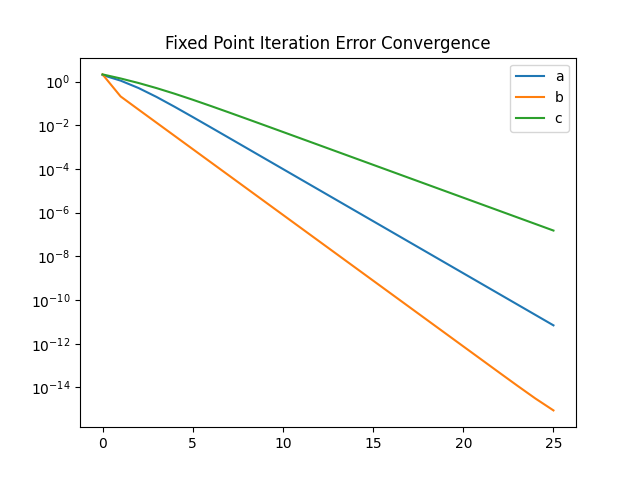
\includegraphics[width=0.8\textwidth]{4.2.2_fig.png}
\end{center}
\begin{verbatim}
0.333340423721603
0.2857142857142857
0.5000000386854939
\end{verbatim}
\end{solution}



\begin{problem}{Q2}
Consider the system:
$$ \begin{cases} 
x_1 - x_2^2 &= 0\\
x^2_1 \qquad & = 1\\
\qquad x^3_2 & = -1.
\end{cases}$$
    \item[(a)] Write the linearization of this overdetermined system of equations at $x^{(0)} = \begin{bmatrix} -1 \\ -1\end{bmatrix}$.

    \vskip0.5cm


    \item[(b)] Write the normal equations of that overdetermined system of linear equations.

    \vskip0.5cm


    \item[(c)] Solving this normal equation may produce a better solution $x^{(1)}\in\mathbb{R}^2$ for the original nonlinear system. Repeating this process would produce a sequence of solutions $x^{(2)},x^{(3)},\dots$. Below is the output of doing 15 steps of this computationally. What kind of convergence rate (if any) is occurring here? Provide a clear and precise justification for your answer.
    
    \footnotesize
    \begin{align*}
        x^{(0)} &= [-1.0, -1.0]\\
        x^{(1)} &= [-0.7049180327868853, -0.7377049180327869]\\
        x^{(2)} &= [-0.5961544668329201, -0.5920469357858523]\\
        x^{(3)} &= [-0.5734364939847171, -0.4880872534988298]\\
        x^{(4)} &= [-0.6126630686880021, -0.352107237762428]\\
        x^{(5)} &= [-0.7346652840213769, 0.0404284117274441]\\
        x^{(6)} &= [-1.074077130433277, -13.962032818418985]\\
        x^{(7)} &= [10.735886119334763, -9.305309168232425]\\
        x^{(8)} &= [5.465161571969174, -6.200949238642323]\\
        x^{(9)} &= [2.9069619580820376, -4.133405178953003]\\
        x^{(10)} &= [1.7440552224433545, -2.7625015427373016]\\
        x^{(11)} &= [1.2759307423154964, -1.8703138738001739]\\
        x^{(12)} &= [1.0889095476973298, -1.3291002276683208]\\
        x^{(13)} &= [1.0161436089776712, -1.0691454883430342]\\
        x^{(14)} &= [1.0007883730394993, -1.0038797134696873]\\
        x^{(15)} &= [1.0000024812781891, -1.0000130644033616]\\
        x^{(16)} &= [1.0000000000278062, -1.0000000001486962]
    \end{align*}
\end{problem}
\begin{solution}
\begin{enumerate}[(a)]
\item The first-order (linear) Taylor expansion gives us a linearization of a multivariate system as $F(\tilde{x}) = F(x) + \nabla F(x)(\tilde{x} - x)$.

Computing the Jacobian and plugging in, we get:
\begin{align*}
    F(x) &= F(x^{0}) + \nabla F(x^{(0)})(\tilde{x} - x^{(0)}) \\
    \begin{bmatrix*}0 \\ 1 \\ -1\end{bmatrix*} &= \begin{bmatrix*}x_1 - x_2^2 \\ x_1^2 \\ x_2^3\end{bmatrix*} + \begin{bmatrix*}1 & -2x_2 \\2x_1 & 0 \\ 0 & 3x_2^2\end{bmatrix*}\left(\tilde{x} - x^{(0)}\right) \\
    \begin{bmatrix*}0 \\ 1 \\ -1\end{bmatrix*} &= \begin{bmatrix*}-1 - (-1)^2 \\ (-1)^2 \\ (-1)^3\end{bmatrix*} + \begin{bmatrix*}1 & -2(-1) \\ 2(-1) & 0 \\ 0 & 3(-1)^2\end{bmatrix*}\left(\tilde{x} - \begin{bmatrix*}-1 \\ -1\end{bmatrix*}\right) \\
    \begin{bmatrix*}0 \\ 1 \\ -1\end{bmatrix*} &= \begin{bmatrix*}-2 \\ 1 \\ -1\end{bmatrix*} + \begin{bmatrix*}1 & 2 \\ -2 & 0 \\ 0 & 3\end{bmatrix*}\left(\tilde{x} - \begin{bmatrix*}-1 \\ -1\end{bmatrix*}\right) \\
    \begin{bmatrix*}0 \\ 1 \\ -1\end{bmatrix*} - \begin{bmatrix*}-2 \\ 1 \\ -1\end{bmatrix*} + \begin{bmatrix*}1 & 2 \\ -2 & 0 \\ 0 & 3\end{bmatrix*}\begin{bmatrix*}-1 \\ -1\end{bmatrix*} &= \begin{bmatrix*}1 & 2 \\ -2 & 0 \\ 0 & 3\end{bmatrix*}\tilde{x} \\
    \begin{bmatrix*} 2 \\ 0 \\ 0\end{bmatrix*} + \begin{bmatrix*}-3 \\ 2 \\-3 \end{bmatrix*} &= \begin{bmatrix*}1 & 2 \\ -2 & 0 \\ 0 & 3\end{bmatrix*}\tilde{x} \\
    \begin{bmatrix*}-1 \\ 2 \\-3 \end{bmatrix*} &= \begin{bmatrix*}1 & 2 \\ -2 & 0 \\ 0 & 3\end{bmatrix*}\tilde{x} \\
\end{align*}
\item The normal equations for an overdetermined linear system are given by: $A^TAx = A^Tb$. For this specific problem, we express this as:
\begin{align*}
    \begin{bmatrix*}1 & -2 & 0 \\ 2 & 0 & 3\end{bmatrix*} \begin{bmatrix*}-1 \\ 2 \\-3 \end{bmatrix*} &= \begin{bmatrix*}1 & -2 & 0 \\ 2 & 0 & 3\end{bmatrix*} \begin{bmatrix*}1 & 2 \\ -2 & 0 \\ 0 & 3\end{bmatrix*}\tilde{x} \\
    \begin{bmatrix*}-5 \\ -11\end{bmatrix*} &= \begin{bmatrix*}5 & 2 \\2 & 13\end{bmatrix*}\tilde{x}
\end{align*}
\item The idea behind Newton's Method is that in the first order linearization, we get that the error term is proportional to the quadratic terms of the Taylor expansion. Thus we should hope to see quadratic convergence in this problem. In practice, we see this convergence in the last few steps as the number of 0s is roughly doubling.
\end{enumerate}
\end{solution}





\end{document}
